\section{Datos}\label{sec:datos}

\textbf{Rendimiento.} Usamos el cierre agrícola municipal del SIAP para cebada grano de temporal en
primavera-verano, de 2003 a 2025~\cite{siap}. Quitamos las cosechas de menos de 50\,ha y los municipios con menos de
5 años de datos. Quedan 1\,942 registros municipio-año de 100 municipios, unos 25 por estado.

\textbf{Unidad de análisis.} La unidad es el municipio. Para cada uno promediamos sus años con una media simple. Cada
municipio tiene entre 5 y 23 años, con mediana de 22. El modelo se ajusta y se evalúa con esos 100 promedios. Los
1\,942 registros no son observaciones independientes, porque los de un mismo municipio se parecen entre sí.

\textbf{Tendencia.} El rendimiento sube en promedio 0.028\,t/ha por año, estimado con los 100 municipios. Esa cifra es
descriptiva. Con ella llevamos cada año al nivel de 2025 antes de promediar, para dibujar los mapas y las
dispersiones. En la validación la pendiente se estima de nuevo en cada partición, solo con los municipios de
entrenamiento, y se suma a la predicción de cada año. Entre particiones con zona de exclusión de 50\,km la pendiente
es inestable y va de 0.013 a 0.050\,t/ha por año. Sin tendencia el RMSE del modelo final sería 0.417\,t/ha en lugar de
0.438. Es decir que la tendencia no mejora la métrica, porque esta compara promedios de todos los años de cada
municipio. El nivel de 2025 tampoco se valida con esa métrica. Con solo los 76 registros de 2025, el error por
registro del modelo final es de 0.88\,t/ha.

\textbf{Cifras repetidas.} El SIAP muchas veces estima una cifra por distrito y la copia a varios municipios. En 1\,036
de los 1\,942 registros (53\,\%) la cifra coincide, a dos decimales, con la de otro municipio del mismo estado y año.
En total, 651 pares de municipios comparten una cifra idéntica en al menos un año. La zona de exclusión de 50\,km
no impide que una cifra repetida quede en el entrenamiento y en la prueba. Con esa zona, 154 de los 651 pares
quedan separados entre ambos conjuntos, y el 10.7\,\% de los registros de prueba conserva un gemelo en el
entrenamiento (38.9\,\% sin zona de exclusión). Al quitar del entrenamiento esos gemelos, el RMSE sube entre 0.001
y 0.005\,t/ha y el orden de los modelos no cambia.

\textbf{Ambiente.} Usamos lluvia de CHIRPS~\cite{chirps}, temperatura máxima (Tmax) y mínima de
CHIRTS-ERA5~\cite{chirts,verdin2020,hersbach2020}, elevación y pendiente del Copernicus DEM~\cite{copdem} y la carta
de suelos del INEGI~\cite{inegi_eda}. Cada variable se promedia solo sobre la agricultura de temporal del
municipio~\cite{inegi_usv}, en los 486 municipios del Marco Geoestadístico~\cite{inegi_mg}.

La Fig.~\ref{fig:mapas_obs} muestra el patrón central. Los municipios con mejor rendimiento están donde el verano es
más fresco, en el oriente de Puebla, Tlaxcala y el centro del Estado de México.

\begin{figure*}[t]
\centering
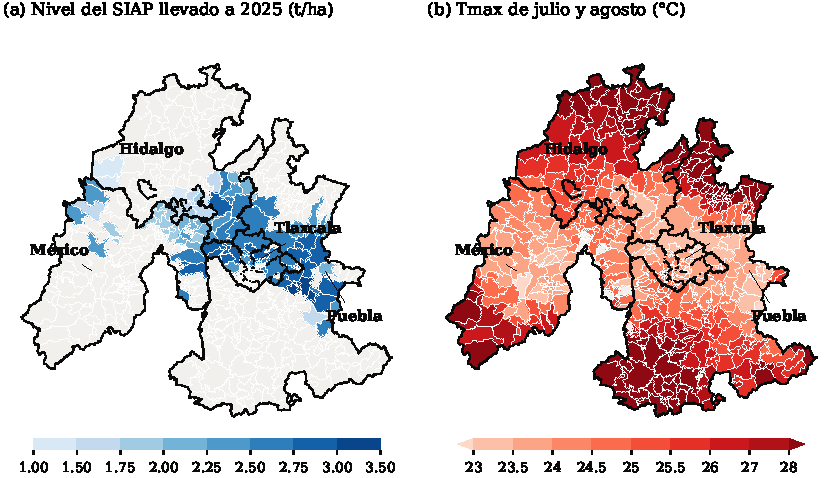
\includegraphics[width=\textwidth]{g_mapas_obs}
\caption{(a) Rendimiento oficial promedio de cada municipio con datos del SIAP, llevado a 2025. (b) Temperatura
máxima promedio de julio y agosto en la agricultura de temporal de cada municipio.}
\label{fig:mapas_obs}
\end{figure*}
